\documentclass[UTF8,titlepage,twocolumn]{ctexart}
\usepackage{amsmath}
\usepackage{caption}
\usepackage{listings}
\usepackage{graphicx}
\pagestyle{plain}
\title{一维二阶Poisson求解}
\date{\today}
\begin{document}
\maketitle	

\lstset{language=Python}



\section{数值算例}
\subsection{Poisson方程}
$
\begin{cases}
Lu = -u''(x) = f(x) \quad x \in G, \\
u(0)=u(\pi)=0
\end{cases}
$ \\
\par
其中f(x) = sin(x), G = [0, $\pi$], 真解为u(x) = sin(x)。
\subsection{变分}

令$v \in C_0^\infty $, 以 v 乘以方程两端得:
$$
\int_0^\pi (Lu - f) v dx = \int_0^\pi (- \frac{\partial^2 u}{\partial x^2} - sin(x)) v dx = 0
$$
\par
由分步积分法得:
$$
\int_0^\pi \frac{\partial u}{\partial x} \frac{\partial v}{\partial x} dx = \int_0^\pi v sin(x) dx
$$
\par 
令a(u,v) = $\int_0^\pi \frac{\partial u}{\partial x} \frac{\partial v}{\partial x} dx$,得原方程变分形式:
$$
a(u,v) = (f,v)
$$

\subsection{剖分}

将区间 G 分成 n 等分, 分点为
$$
x_i = ih \quad i = 0,1,...,n,
$$
\par 
其中 h = $\frac{\pi}{n}$ , 剖分单元$I_i = [x_{x-1}, x_i] $.

\subsection{构造基函数}

基函数选取山形函数
$$
\begin{cases}
	\phi_0(x) = \begin{cases}
					1 - \frac{x - x_0}{h_1}, \quad x_0 \le x \le x_1, \\
					0, 						 \quad \mbox{其他}.
				\end{cases} \\
	\phi_i(x) = \begin{cases}
					1 + \frac{x - x_i}{h_i},     \quad x_{i-1} \le x \le x_i,    \\
					1 - \frac{x - x_i}{h_{i+1}}, \quad x_i     \le x \le x_{i+1} \\
					0,                           \quad \mbox{其他},	
				\end{cases} \\
	\phi_n(x) = \begin{cases}
					1 + \frac{x - x_n}{h_n}, \quad x_{n-1} \le x \le x_n, \\
					0,						 \quad \mbox{其他}
				\end{cases}
\end{cases}
$$
\par 
借助仿射变换,及[0,1]上的标准山形函数
$$
\varepsilon = F_i(x) = \frac{x - x_{i-1}}{h_i}, \quad \quad
N_0(\varepsilon) = 1 - \varepsilon, N_1(\varepsilon) = \varepsilon, 
$$
\par 
则对基函数 i = 1,2,...,n-1,基函数可写成:

$$
\phi_i(x) = 
\begin{cases}
	N_0(\varepsilon), \quad \varepsilon = \frac{x - x_i}{h_{i+1}}, \quad x_i     \le x \le x_{i+1} \\
	N_1(\varepsilon), \quad \varepsilon = \frac{x - x_{i-1}}{h_i}, \quad x_{i-1} \le x \le x_i \\
	0, \quad \quad                                                 \quad \mbox{其他},
\end{cases}
$$
\par 
而
$$
\phi_0(x) = \begin{cases}
				N_0(\varepsilon), \quad \varepsilon = \frac{x - x_0}{h_1}, \quad x_0 \le x \le x_1, \\
				0, \quad \quad                                       \quad \mbox{其他}
			\end{cases}\\
$$
\par
$$
\phi_n(x) = 
\begin{cases}
	N_1(\varepsilon), \quad \varepsilon = \frac{x - x_{n-1}}{h_n}, \quad x_{n-1} \le x \le x_n, \\
	0, \quad \quad          									   \quad \mbox{其他}. 
\end{cases}
$$

\subsection{形成有限元方程}

设数值解$u_h = \sum_{i=0}^n c_i \phi_i $, 由边值条件得$c_0 = c_n = 0, \mbox{且}c_i = u_i, i=1,...,n-1$.
带入变分形式得有限元方程:
$$
\sum_{j=1}^{n-1} a(\phi_j, \phi_i) c_j = (f, \phi_i), \quad i = 1, 2, ... , n-1
$$
\par 
其矩阵形式为
$$ K \bar{c} = \bar{b} $$
其中
$$
\begin{matrix}
K = \begin{bmatrix}
		a(\phi_1,\phi_1) & a(\phi_1,\phi_2) & ... & a(\phi_1,\phi_{n-1}) \\
		a(\phi_2,\phi_1) & a(\phi_2,\phi_2) & ... & a(\phi_2,\phi_{n-1}) \\
		\vdots           & \vdots           &     & \vdots  			 \\
		a(\phi_{n-1},\phi_1) & a(\phi_{n-1},\phi_2) & ... & a(\phi_{n-1},\phi_{n-1})
	\end{bmatrix}, \\ \\
\bar{c} = (c_1, c_2, ... , c_{n-1})^T \\ \\
\bar{b} = ((f,\phi_1), (f,\phi_2), ... , (f,\phi_{n-1}))^T.
\end{matrix}
$$

\subsection{从单元刚度矩阵组装总刚度矩阵}
令$ v_h = \sum_{i=0}^{n} v_i \phi_i $,双线性泛函 $a(u_h,v_h)$ 在剖分单元$ I_i = [x_{i-1},x_i] $ 上的限制为

$$
	a(u_h,v_h) = (v_{i-1},v_i) K^{I_i} 
	\begin{pmatrix}
		u_{i-1} \\
		u_i
	\end{pmatrix}
$$

其中
$$
K^{I_i}:= \begin{bmatrix}
		  		a_{i-1,i-1}^{I_i} & a_{i-1,i}^{I_i} \\
		  		a_{i,i-1}^{I_i}   & a_{i,i}^{I_i}
		  \end{bmatrix} =
	  \begin{bmatrix}
	  	a(N_0,N_0)_{I_i} & a(N_0,N_1)_{I_i} \\
	  	a(N_1,N_0)_{I_i} & a(N_1,N_1)_{I_i}
	  \end{bmatrix}
$$
为单元刚度矩阵
\\ \par
泛函$(f,v_h)$在剖分单元$I_i$上的限制为
$$
	(f,v_h)_{I_i} = (v_{i-1},v_i) b^{I_i}
$$

其中
$$
	b^{I_i} = \begin{pmatrix}
				b_{i-1}^{I_i} \\
				b_i^{I_i}
			  \end{pmatrix} ==
		      \begin{pmatrix}
		      	(f,N_0)_{I_i} \\
		      	(f,N_1)_{I_i}
		      \end{pmatrix}
$$
为单元载荷向量。
\\ \par 
将$K^{I_i}$扩展成n $\times$ n 矩阵,第i-1行和第i行和第i-1列和第i列就是$K^{I_i}$的四个元素,其余全为零,则总刚度矩阵 
$$ 
	K = \sum_{i=1}^{n-1} K^{I_i}
$$
以同样的方式得到总载荷向量
$$
	\bar{b} = \sum_{i=1}^{n-1} b^{I_i}
$$

\subsection{实验结果}

当剖分次数n=5时,得到数值解与真解如下图
\begin{figure}[hb]
	\centering
	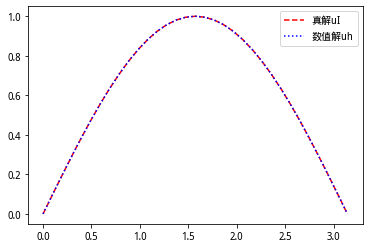
\includegraphics[height=5cm,width=7cm]{../image/Poisson1d.png}
	\caption{}
	\label{SampleOfDatasets}
\end{figure}
\\ \\ \\ \\ \\ \\
改变剖分步长h得到其与误差二范数e的关系如下表

\begin{table}[!ht]
	\centering
	\caption{}%剖分次数-误差二范数
	\begin{tabular}{|c|c|} \hline
		h & e \\ \hline
		1.57 & 1.63e-07 \\ \hline
		0.78 & 8.29e-10 \\ \hline
		0.39 & 4.48e-12 \\ \hline
		0.19 & 2.11e-14 \\ \hline
		0.09 & 1.33e-14 \\ \hline
	\end{tabular}
\end{table}

\begin{figure}[hb]
	\centering
	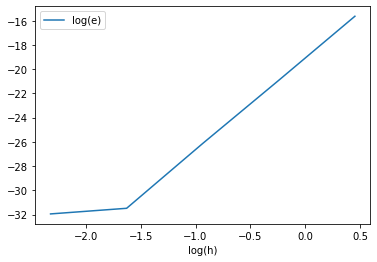
\includegraphics[height=5cm,width=7cm]{../image/Poisson1d_误差_步长.png}
	\caption{}
\end{figure}

\end{document}